\section{Circuit Design}
	\begin{figure}[ht!]
	\begin{tikzpicture}
		[->,>=stealth',semithick]	
		\node[rectangle,draw] (r0) at (0, 0) {Photodiode};
		\node[rectangle,draw,text width=1cm, align=center] (r1) at (-1, -2) {RED LED};
		\node[rectangle,draw,text width=1cm, align=center] (r2) at (1, -2) {IR LED};	
		\node[rectangle,draw,text width=1cm, align=center] (r3) at (0, -4) {LED Driver};
		\node[rectangle,draw,text width=3cm, align=center] (r4) at (4, 0) {Transimpedance Amplifier};
		\node[rectangle,draw,text width=2cm, align=center] (r5) at (8, 0) {Difference  Amplifier};
		\node[rectangle,draw,text width=3cm, align=center] (r6) at (8, -2) {Programmable Gain Amplifier};
		\node[rectangle,draw,text width=1cm, align=center] (r7) at (8, -4) {$\mu$C ADC};
		\node[rectangle,draw,text width=1cm, align=center] (r8) at (2, -4) {$\mu$C};
		\node[rectangle,draw,text width=1cm, align=center] (r9) at (5, -2) {$\mu$C};
		
		\path (r1) edge (r0);
		\path (r2) edge (r0);
		\path (r3) edge (r1) 
		edge (r2);
		\path (r0) edge (r4);
		\path (r4) edge (r5);
		\path (r5) edge (r6);
		\path (r6) edge (r7);
		\path (r8) edge (r3);
		\path (r9) edge (r6);
		
	\end{tikzpicture}
	\caption{System Block Diagram}
	\end{figure}

	Referring the Block diagram, subsections are divided below that show the circuit and corresponding oscilloscope trace outputs.
	
	\subsection{Front End}	
	
		\subsubsection{Transimpedance Stage}
		
			Photodiode's current is needed to be converted to a proportional voltage so that ultimately the microcontoller can convert the voltage to a digital value using an ADC for calculation of SpO\textsubscript{2}. A simple Transimpedance Amplifier configuration was used to achieve this:
			
			\begin{figure}[ht!]\centering
				\begin{circuitikz}[american] 
					\draw
					
					(2,3) node[op amp,yscale=-1] (opamp) {}
					(opamp.down) -- +(0,0.3) node[vcc]{Vcc}
					(opamp.up) -- +(0,-0.3) node[ground]{}
					(0,0) node[ground]{} to[pDo, l^=$D$, f^=$I$]  (0,2.5) to (opamp.-)
					(opamp.+) node[ground]{}
					(opamp.-) -- ++(0,-1.7) -- ++(0.5,0)
					to [R, l^=$R_1$] ++(1.5,0) -- ++(0.4,0) to (opamp.out)
					(opamp.-)  ++(0,-1.7) -- ++(0,-1.3) -- ++(0.5,0) 
					to [C, l^=$C_1$]  ++(1.5,0) -- ++(0.4,0) -- ++(0,1.3) 
					(opamp.out) -- ++(1,0) to [open,v=$V_1$,o-o] ++(0,-3) node[ground]{};
					
				\end{circuitikz}
			\end{figure}
			
		
			As per led's intensity, if a current of 10$\mu$A is produced in the photodiode, and R = 100K$\Omega$, according to Ohm's law, $V_1$ = 1 V. Capacitor is used for low-pass filtering of the pulse. Cut off frequency would be:
		
		
			\begin{equation}	
				F_c = \frac{1}{2\pi R_1C_1}
			\end{equation}
		
			If R\textsubscript{1}=576K$\Omega$, C\textsubscript{1} = 33pF, 
			
			\[	
			F_c \approx \SI{8.3}{\kilo\hertz}
			\]
		
			\begin{figure}[ht!]
				\centering
				\subfloat[V\textsubscript{1} 
				]{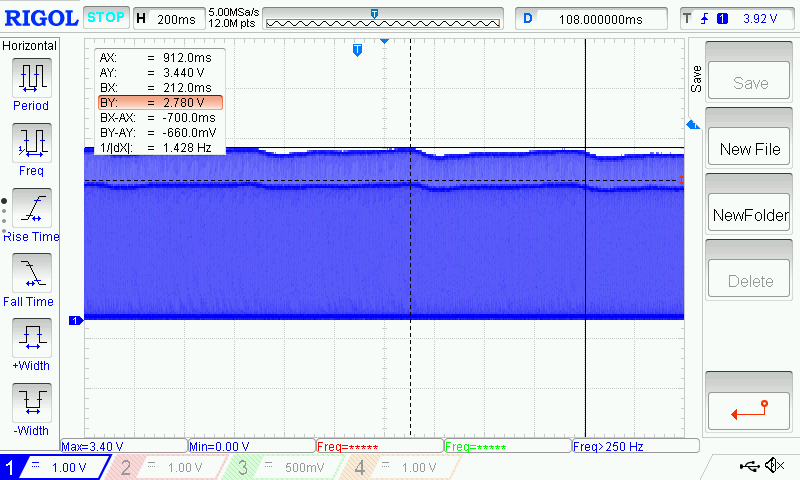
\includegraphics[width=0.9\textwidth]{../common/circuit/itov.png}}
				\hfill
				\subfloat[V\textsubscript{1} zoomed in 
				]{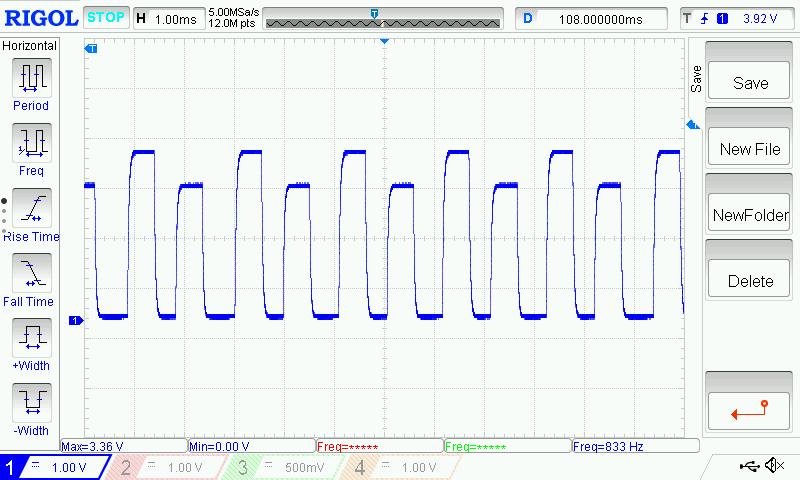
\includegraphics[width=0.9\textwidth]{../common/circuit/itov_zoom.png}
				\label{fig:itov}}
				\caption{V\textsubscript{1} Oscilloscope trace (Red \& IR pulsed sequentially) }
			\end{figure}
		
			Since LEDs are pulse on-off at a fast rate sequentially the pulse would look like a square wave. We need to use a pulse frequency less than 1/10\textsuperscript{th} of this cut-off to pulse the LEDs so that the square wave with all its high-frequency components is clearly visible and not filtered out.
			
			\[	
			F_p = \SI{500}{\hertz}
			\]
					
		
			It can be seen in traces, 2 PPG signals are observable, riding on a DC level. Higher amplitude one is a result of ir led pulsing, while lower amplitude is from red led. Since the peaks correspond to heart rate, in this case as per trace, it measures out to be 1.42/sec or 85BPM. Individual pulses which construct the signal can be seen in Figure \ref{fig:itov}. Amplitude of detected red signal is lower than ir and that is due to:
			
			\begin{itemize}
				
				\item Higher intensity of ir led due to higher ir current.
				\item Photodiode's red sensitivity is 80\% of ir sensitivity. 
				\item Ir penetrates into skin deeper than red, hence a better ir response is visible at photodiode\cite{penetrate}.
				
			\end{itemize}		
			Hence to obtain a suitable response, it is important to increase led intensity until it reaches a required level so that the PPG signal has a higher amplitude.	
			
		\subsubsection{Difference Amplifier}
		
			PPG signal needs to be amplified to a suitable level so that full scale ADC range can be utilized to better digitize the signal. Right now, amplitude of PPG signal is quite low and DC level is higher. We are not bothered by the DC anymore, $\mu$C can read it and store for R value calculation, we only need to amplify the AC part which is an envelope of the signal. Direct amplification would lead to gain of the DC level as well, as the required signal is riding on top of it. This will saturate the opamp and amplification level range will be quite low. 
			
			\begin{figure}[ht!]
				\centering
				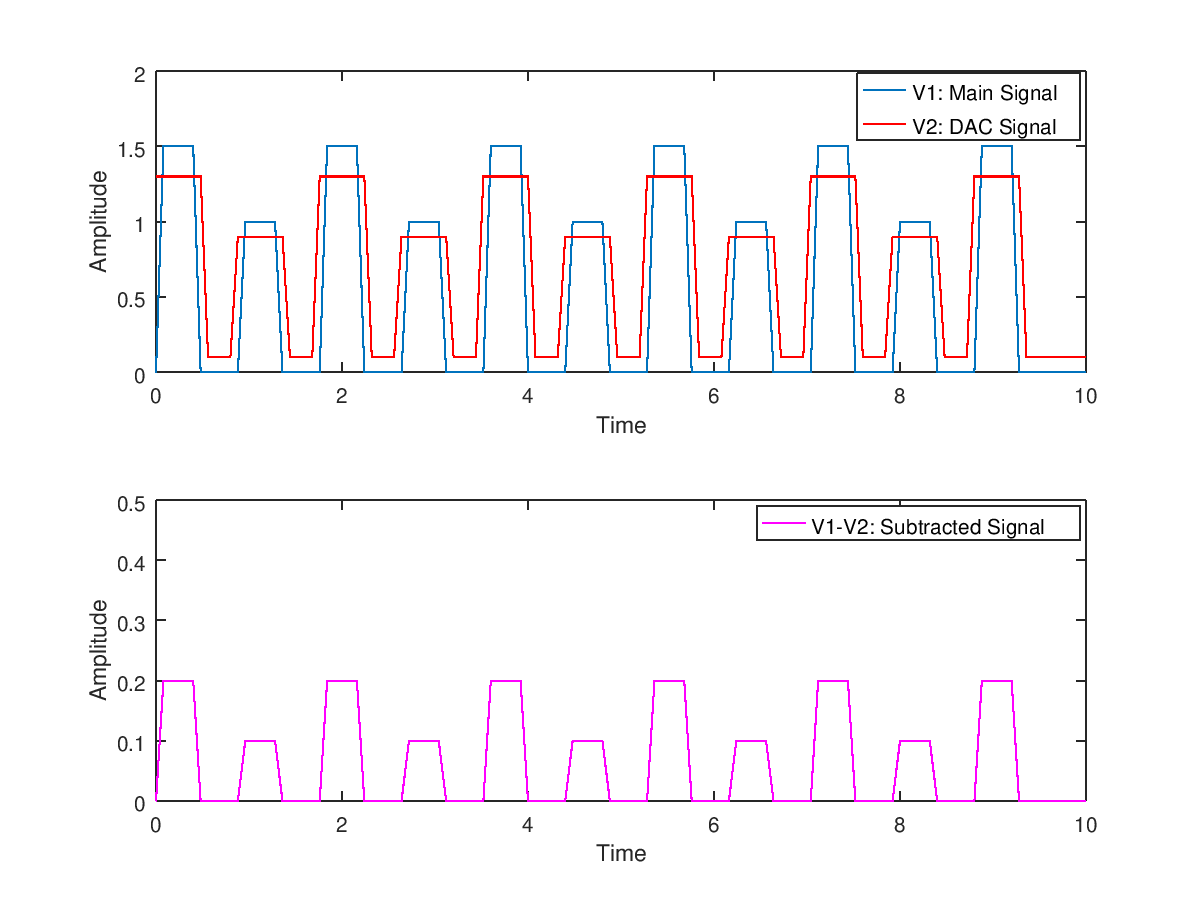
\includegraphics[width=0.8\textwidth]{../common/circuit/diff.png}
				\caption{Effect of Difference Amplifier}
				\label{fig:diff}
			\end{figure}	
			
			If we can subtract the DC level from entire signal, only AC would remain which can be easily amplified further at higher levels. A Difference amplifier along with a 8bit Digital to analog converter (DAC) generating the DC cancellation signal can be used here. Since red and ir have different levels, separate DC levels are generated by DAC in sync with the pulsed frequency.\medskip 
			
			As shown in Figure \ref{fig:diff} a plot generated in Octave demonstrates subtraction of required signal and diff signal. This difference can then be amplified further. Pulse width of diff signal is slightly larger than required signal so that there are no spikes on edges in output signal. Also the lower level of diff signal is slightly above 0V to allow the difference to always be negative in low states and since negative supply is grounded, output would be 0V here.
			
			\begin{figure}[ht!]\centering
				\begin{circuitikz}[american] 
					\draw
					
					(4,3) node[op amp,yscale=-1] (opamp) {}
					(opamp.down) -- +(0,0.3) node[vcc]{Vcc}
					(opamp.up) -- +(0,-0.3) node[ground]{}
					(opamp.-) to [R, l^=$R_1$] ++(-2,0) node[label={left:$V_{dac1}$}] {}
					(opamp.+) to [R, l^=$R_1$] ++(-2,0) node[label={left:$V_1$}] {}
					(opamp.+) to [R, l^=$R_1$] ++(0,2) node[ground,rotate = 90]{}
					(opamp.-) -- ++(0,-1.7) -- ++(0.5,0)
					to [R, l^=$R_1$] ++(1.5,0) -- ++(0.4,0) to (opamp.out)
					(opamp.out) -- ++(1,0) to [open,v=$V_2$,o-o] ++(0,-3) node[ground]{};
			
				\end{circuitikz}
			\end{figure}
			


			\[
				V_2 = \frac{R_1}{R_1}(V_1 - V_{dac1})
			\]
			
			
			For $R_1 = 10K$,
			
			\[
				V_2 \approx V_1 - V_{dac1}
			\]
			
						
		\subsubsection{Programmable Gain Amplifier}
		
			It becomes necessary to amplify the signal as skin tone, improper finger contact with sensor or any skin pigmentation\cite{skin} can cause attenuation in signal leading to low amplitudes. This stage provides selectable variable gain which can be set by microcontroller.
			
			$\mu$C would determine what level of further amplification is required and drive the respective pin high so that resistor value would get selected.
			
			
			\begin{figure}[ht!]\centering
				\begin{circuitikz}[american] 
					\draw
						(2,3) node[op amp,yscale=-1] (opamp) {}
						(opamp.down) -- +(0,0.3) node[vcc]{Vcc}
						(opamp.up) -- +(0,-0.3) node[ground]{}
						(opamp.+) to ++(-2,0) node[label={left:$V_{in}$}] {}
						(opamp.-) -- ++(0,-1.7) -- ++(1,0)
						to [R, l^=$10K$] ++(1,0) -- ++(1,0) -- ++(0,2.2) to (opamp.out)
						(opamp.-) ++(0,-1.7) -- ++(0,-1.5) to [R, l^=$10K$] ++(0,-1) -- ++(0,-0.5)
						++(0,-0.5) node[npn] (Q1){}
						(Q1.E) node[ground]{}
						(Q1.B) to [R, l^=$4.7K$] ++(-1.5,0) node[label={left:S1}] {}
						
						(opamp.-) ++(0,-1.7) ++(0,-0.75) -- ++(3.5,0) -- ++(0,-0.75)		
						to [R, l^=$4.7K$] ++(0,-1) -- ++(0,-0.5)
						++(0,-0.5) node[npn] (Q2){}	
						(Q2.E) node[ground]{}	
						(Q2.B) to [R, l^=$4.7K$] ++(-1.5,0) node[label={left:S2}] {}
						
						(opamp.-) ++(0,-1.7) ++(0,-0.75) ++(2,0) -- ++(5,0) -- ++(0,-0.75)		
						to [R, l^=$2.35K$] ++(0,-1) -- ++(0,-0.5)
						++(0,-0.5) node[npn] (Q3){}	
						(Q3.E) node[ground]{}	
						(Q3.B) to [R, l^=$4.7K$] ++(-1.5,0) node[label={left:S3}] {};
						
						
				 \end{circuitikz}
			\end{figure}	
	
			\begin{center}
				\begin{tabular}{ |c|c|} 
					\hline
					\textbf{Switch} & \textbf{Gain}   \\ 
					\hline
					all off & 1 	\\ 
					\hline
					S1 & 2  		\\ 
					\hline
					S2 & 3  		\\ 
					\hline
					S1+S2 & 4  		\\ 
					\hline
					S3 & 5  		\\ 
					\hline
					S1+S3 & 6	  	\\ 
					\hline
					S2+S3 & 7  		\\ 
					\hline
				\end{tabular}
			\end{center}
		
	
	\subsection{LED Driver}

	
		As discussed previously, the detected signal levels can be very low after I to V stage. LED Driver needs to increase current to the leds as required. Following circuit is used as a voltage controlled current source, voltage is set by the DAC as instructed by the $\mu$C.
		
		\begin{figure}[ht!]\centering
			\begin{circuitikz}[american] 
				\draw
				
				(4,3) node[npn] (Q1){}
				(Q1.E) to [R, l^=20] ++(0,-1.5) node[ground]{}
				(Q1.B) to [R, l^=4.7K] ++(-1.5,0) node[label={left:$V_{dac2}$}] {}
				(Q1.C) -- ++(-1,0) -- ++(0,0.5) ++(0,0.5)  node[npn] (Q2){}
				(Q2.B) to [R, l_=10K] ++(-1.5,0) node[label={left:Red pulse}] {}
				(Q2.C) -- ++(0,1) node[]{} ++(0,0.2) node[]{Red cathode}
				(Q1.C) -- ++(1,0) -- ++(0,0.5) ++(0,0.5) node[npn,xscale=-1] (Q3){}
				(Q3.B) to [R, l^=10K] ++(1.5,0) node[label={right:IR pulse}] {}
				(Q3.C) to ++(0,1) node[]{} ++(0,0.2) node[]{Ir cathode};
			\end{circuitikz}
		\end{figure}
		
		
		Leds get activated by a single bridge configuration, whenever red/ir pulse is active, corresponding red/ir leds get active (led anodes connected to Vcc). Amount of current would depend on $V_{dac2}$ \& $R_1$.
		
		$V_{dac2}$ is also set individually for red and ir as per the pulsed frequency. If intensity is not sufficient for signal detection, it is necessary to increase $V_{dac2}$. $\mu$C would determine the thresholds and modulate the control voltage accordingly.
	
		Shown below is final output after the PGA stage.
		The gained up PPG signal is clearly visible for both red and ir which is at a suitable level for ADC capture and usage in algorithms for calculations.
	
	
	\begin{figure}[ht!]
		\centering
		\subfloat[Final output - green, V\textsubscript{1} - blue
		]{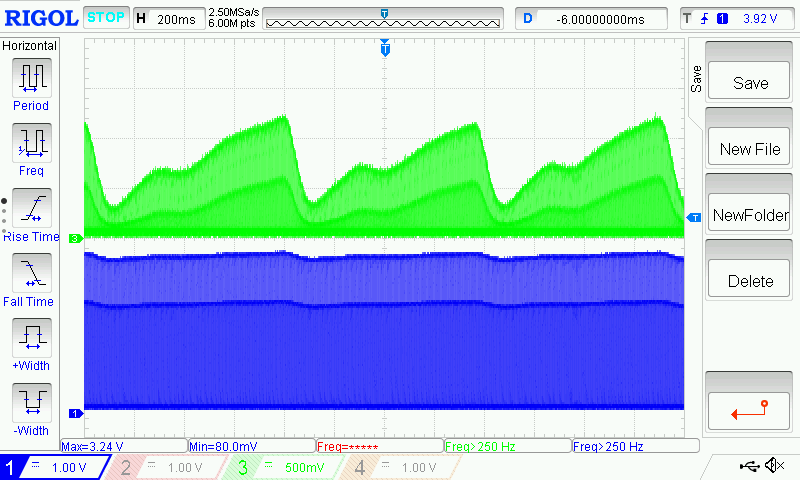
\includegraphics[width=1\textwidth]{../common/circuit/final_out.png}}
		\hfill
		\subfloat[Final output measurement
		]{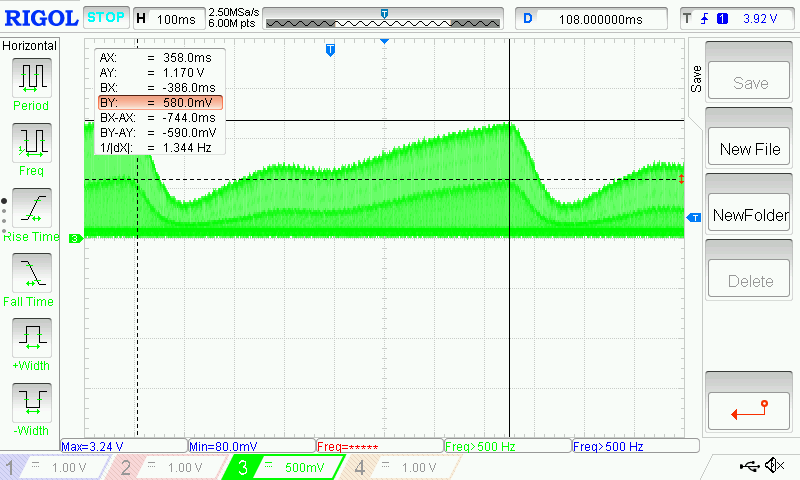
\includegraphics[width=1\textwidth]{../common/circuit/final_out_meas.png}}
		\caption{Final output}
	\end{figure}		
		